% left planar triangle + arrow + right folded tetrahedron-like figure
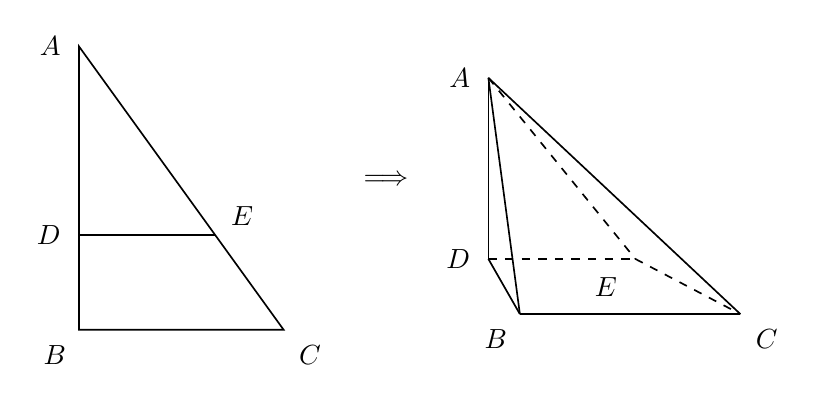
\begin{tikzpicture}[x=1cm,y=1cm,line width=.6pt,font=\normalsize]
% left panel: right triangle ABC, B bottom-left, C bottom-right, A top-left
\coordinate (A) at (0,3.6);
\coordinate (B) at (0,0);
\coordinate (C) at (2.6,0);
\coordinate (D) at (0,1.2);
\coordinate (E) at (1.7333333333,1.2000000000);
\draw (A) -- (B) -- (C) -- cycle;
\draw (D) -- (E);
\node[left,xshift=-3pt] at (A) {$A$};
\node[left,xshift=-3pt] at (D) {$D$};
\node[below left,xshift=-1pt,yshift=-2pt] at (B) {$B$};
\node[above right,xshift=2pt] at (E) {$E$};
\node[below right,xshift=2pt,yshift=-2pt] at (C) {$C$};
% arrow
\node at (3.9,1.9) {$\Longrightarrow$};
% right panel: folded along DE, base plane y=0 with D,B,C,E; apex A above D
\coordinate (rD) at (5.2,0.9);
\coordinate (rB) at (5.6000000000,0.2000000000);
\coordinate (rC) at (8.4,0.2);
\coordinate (rE) at (7.0666666667,0.9000000000);
\coordinate (rA) at (5.2000000000,3.2000000000);
\draw (rB) -- (rC);
\draw (rD) -- (rB);
\draw[dashed] (rD) -- (rE);
\draw[dashed] (rE) -- (rC);
\draw (rA) -- (rD);
\draw (rA) -- (rB);
\draw (rA) -- (rC);
\draw[dashed] (rA) -- (rE);
\node[left,xshift=-3pt] at (rA) {$A$};
\node[left,xshift=-3pt] at (rD) {$D$};
\node[below left,xshift=-1pt,yshift=-2pt] at (rB) {$B$};
\node[below left=3pt] at (rE) {$E$};
\node[below right,xshift=2pt,yshift=-2pt] at (rC) {$C$};
\end{tikzpicture}
